\section{Auswertung}
\label{sec:auswertung}

Im Anschluss werden die aufgenommenen Messwerte ausgewertet.

\subsection{Energiekalibration und Bestimmung der Vollenergienachweiswahrscheinlichkeit}
\label{sec:auswertung1}

Das aufgenommene Spektrum der Eu-152 Quelle ist in der Abbildung \ref{fig:plot1}
dargestellt. Die Anzahl der Impulse wurden für eine bessere Darstellbarkeit logarithmisch abgebildet. 

\begin{figure}[H]
    \centering
    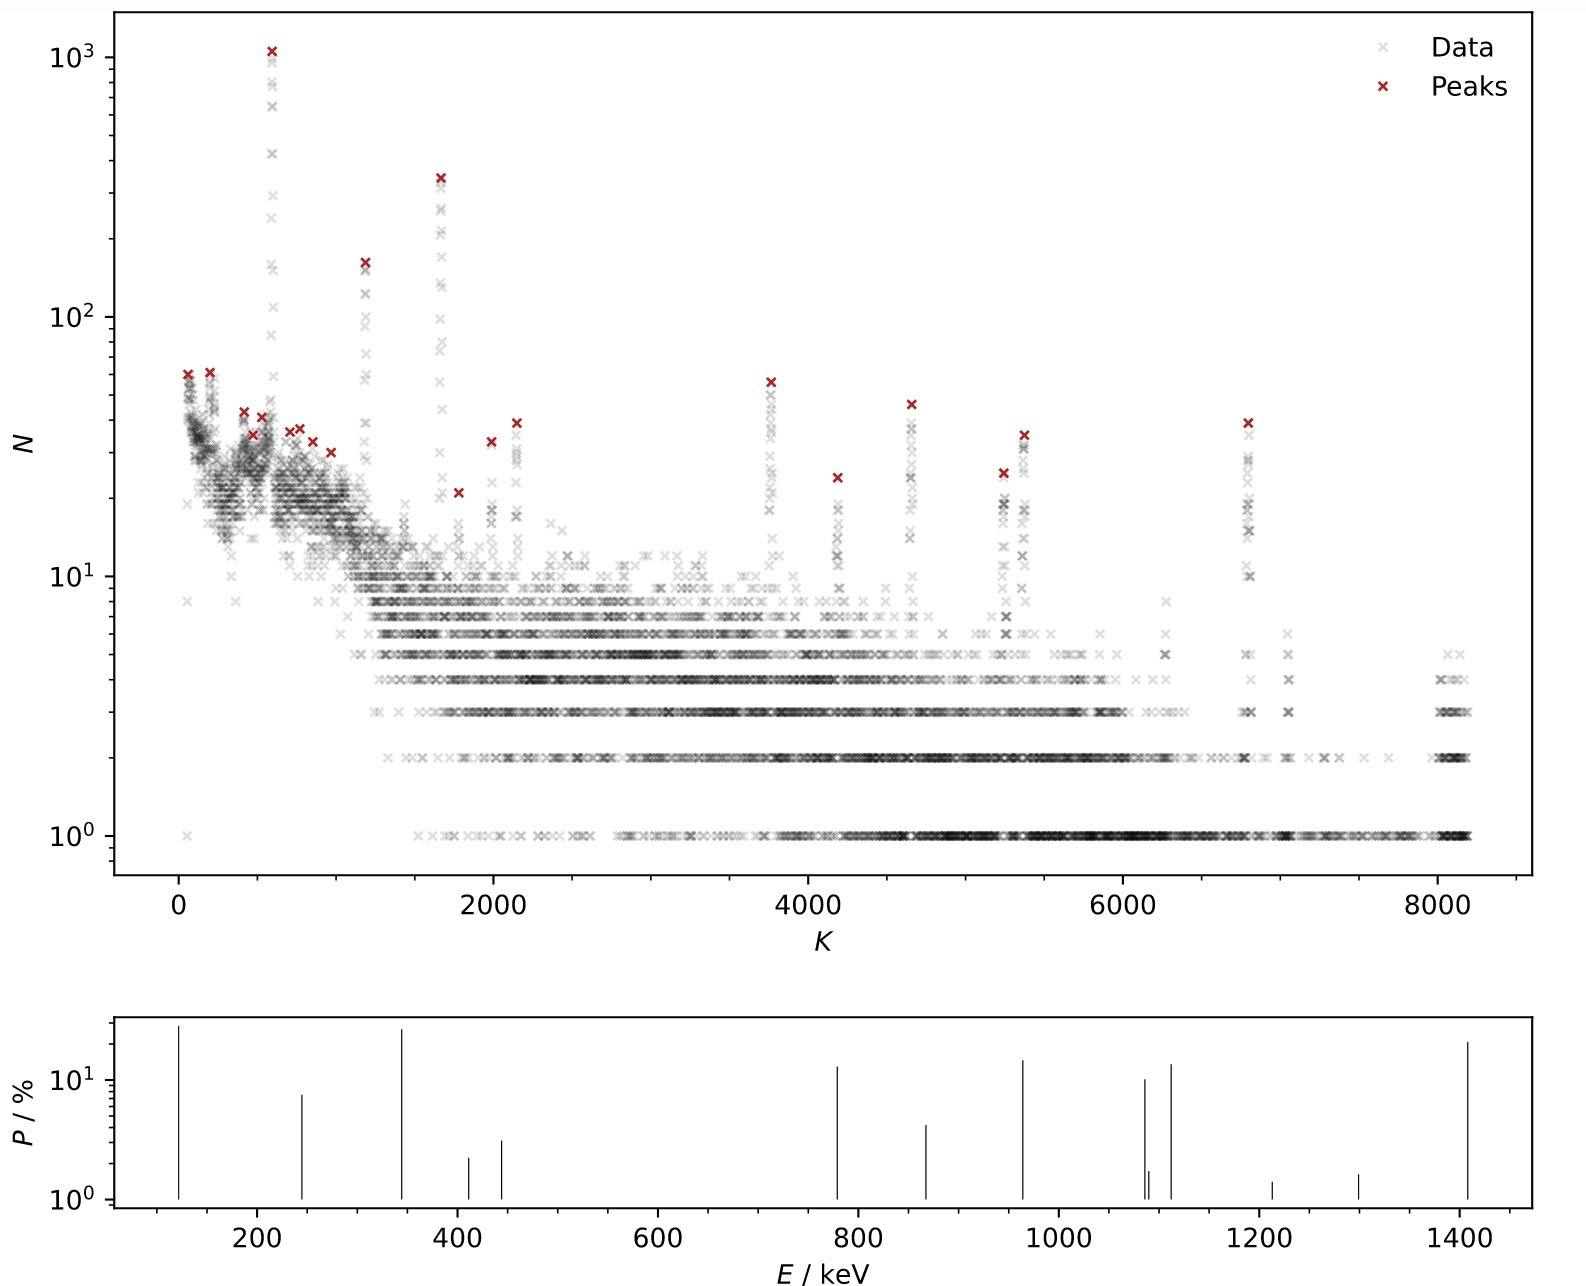
\includegraphics[width=0.9\textwidth]{content/plots/plot1.jpg}
   \caption{Gammaspektrum des Eu-152 Strahlers.}
    \label{fig:plot1}
\end{figure}

Die Photopeaks werden mit dem SciPy Paket find-peaks ermittelt und rot markiert.
Unter dem Spektrum befinden sich die Emissionsenergien des Gammastrahlers, welche zum Abgleichen verwendet werden.
Die Emissionsenergien von Eu-152 sind in der Abbildung \ref{fig:euE} gegeben.

\begin{figure}[H]
    \centering
    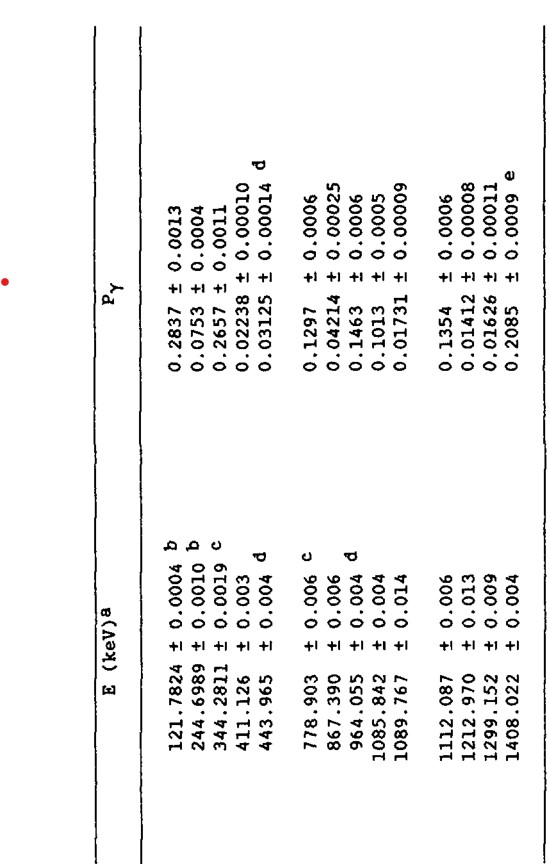
\includegraphics[angle=270,width=0.6\textwidth]{content/grafik/euenergien.jpg}
    \caption{Die Emissionsenergien von Eu-152. \cite{Kalibration}}
    \label{fig:euE}
\end{figure}

Nun werden die zugeordneten Emissionsenergien gegen die Kanäle aufgetragen.
Anschließend wird eine lineare Ausgleichsgerade der Form 
\begin{equation*}
    a \cdot K + b
\end{equation*}
an die Werte angelegt. $K$ bezeichnet dabei die Kanalnummer.
Die Ausgleichsgerade ist in der Abbildung \ref{fig:plot2}
zu sehen.

\begin{figure}[H]
    \centering
    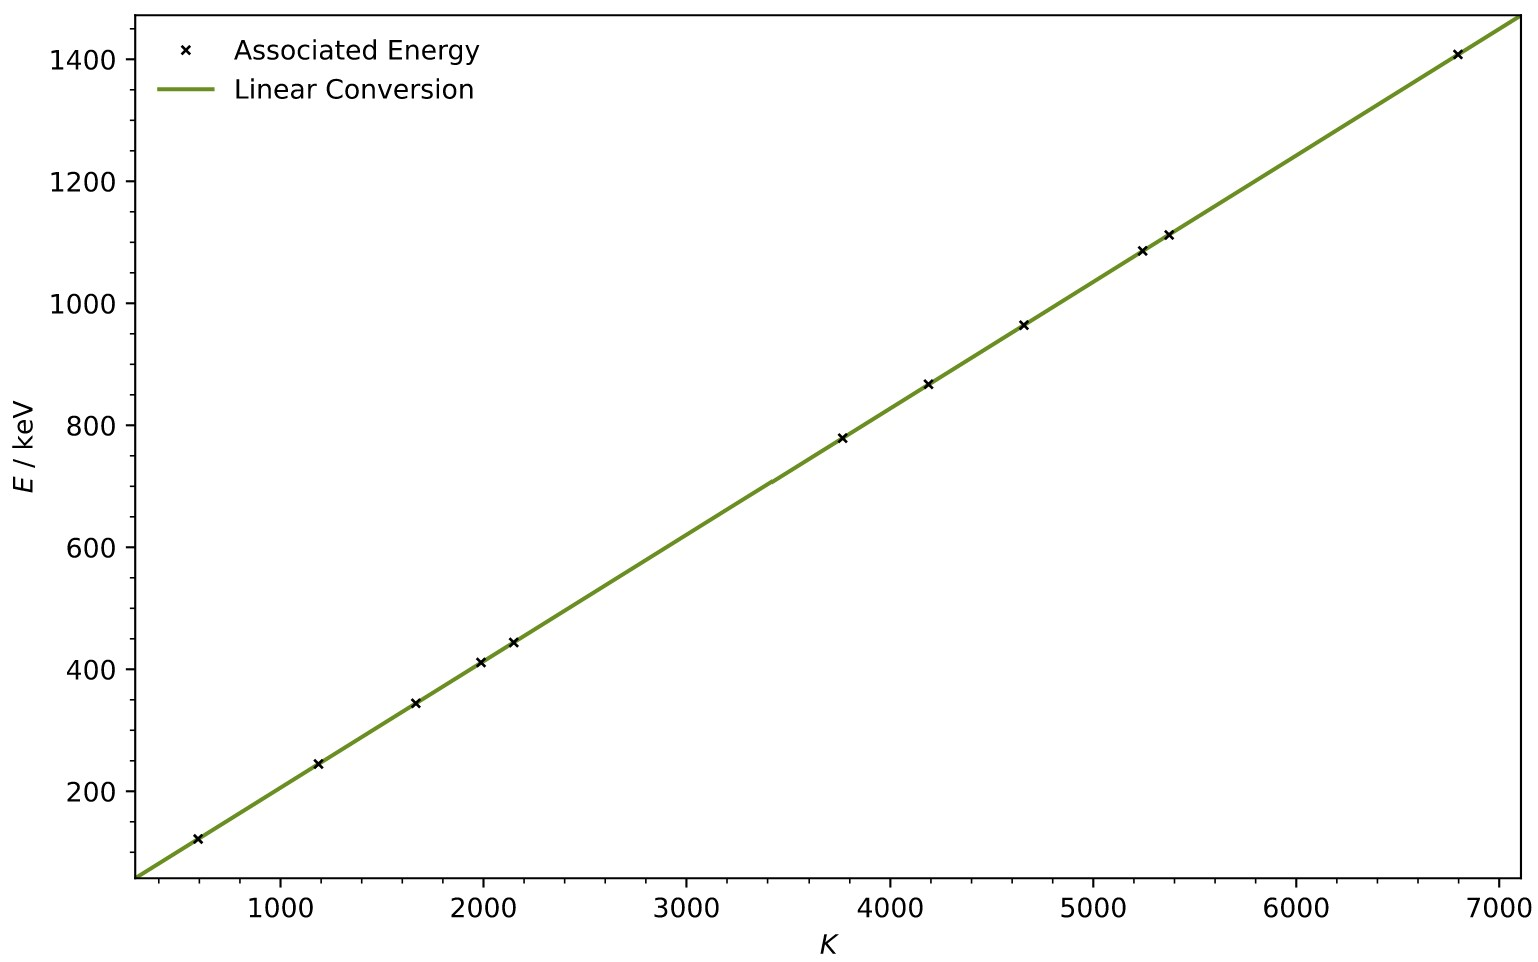
\includegraphics[width=0.8\textwidth]{content/plots/plot2.jpg}
    \caption{Ausgleichsrechnung der Energiekalibration.}
    \label{fig:plot2}
\end{figure}

Für die Parameter ergeben sich die Werte
\begin{align*}
    a   &= \qty{0.2073+-0.0001}{\kilo\eV} \\
    b   &= \qty{-1.3399 +- 0.2191}{\kilo\eV}.
\end{align*}

Für die Energiekalibration ergibt sich demnach
\begin{equation*}
    E\left(K\right) = \qty{0.2073+-0.0001}{\kilo\eV} \cdot K + \qty{-1.3399 +- 0.2191}{\kilo\eV}.
\end{equation*}

Zur Verdeutlichung der Zuordnung der Emissionswahrscheinlichkeiten wurde das Spektrum von Eu-152 mit der Energieskala erneut erstellt und
wird in der Abbildung \ref{fig:plot3}
abgebildet.

\begin{figure}[H]
    \centering
    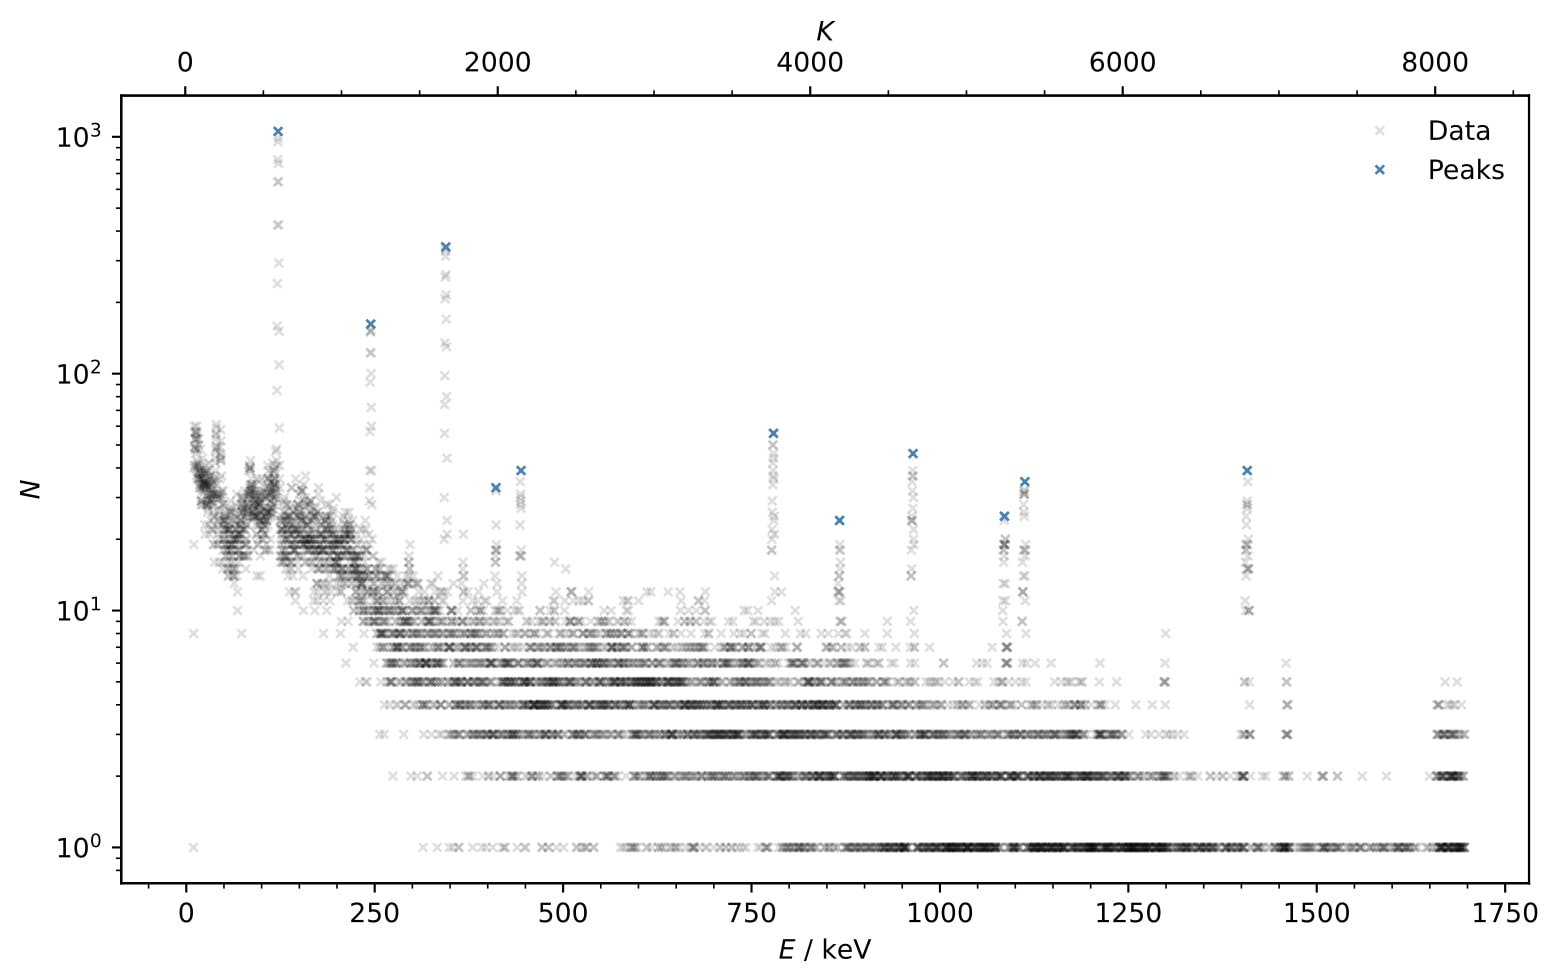
\includegraphics[width=0.8\textwidth]{content/plots/plot3.jpg}
   \caption{Gammaspektrum des Eu-152 Strahlers mit zusätzlicher Energieskala.}
   \label{fig:plot3}
\end{figure}

An die Full Energy Peaks wird jeweils eine Gaußfunktion gefitet. In der Abbildung \ref{fig:plot4} ist für den Peak bei $E$ = \qty{122}{\kilo\eV}
die Gaußkurve und die Messwerte abgebildet.

\begin{figure}[H]
    \centering
    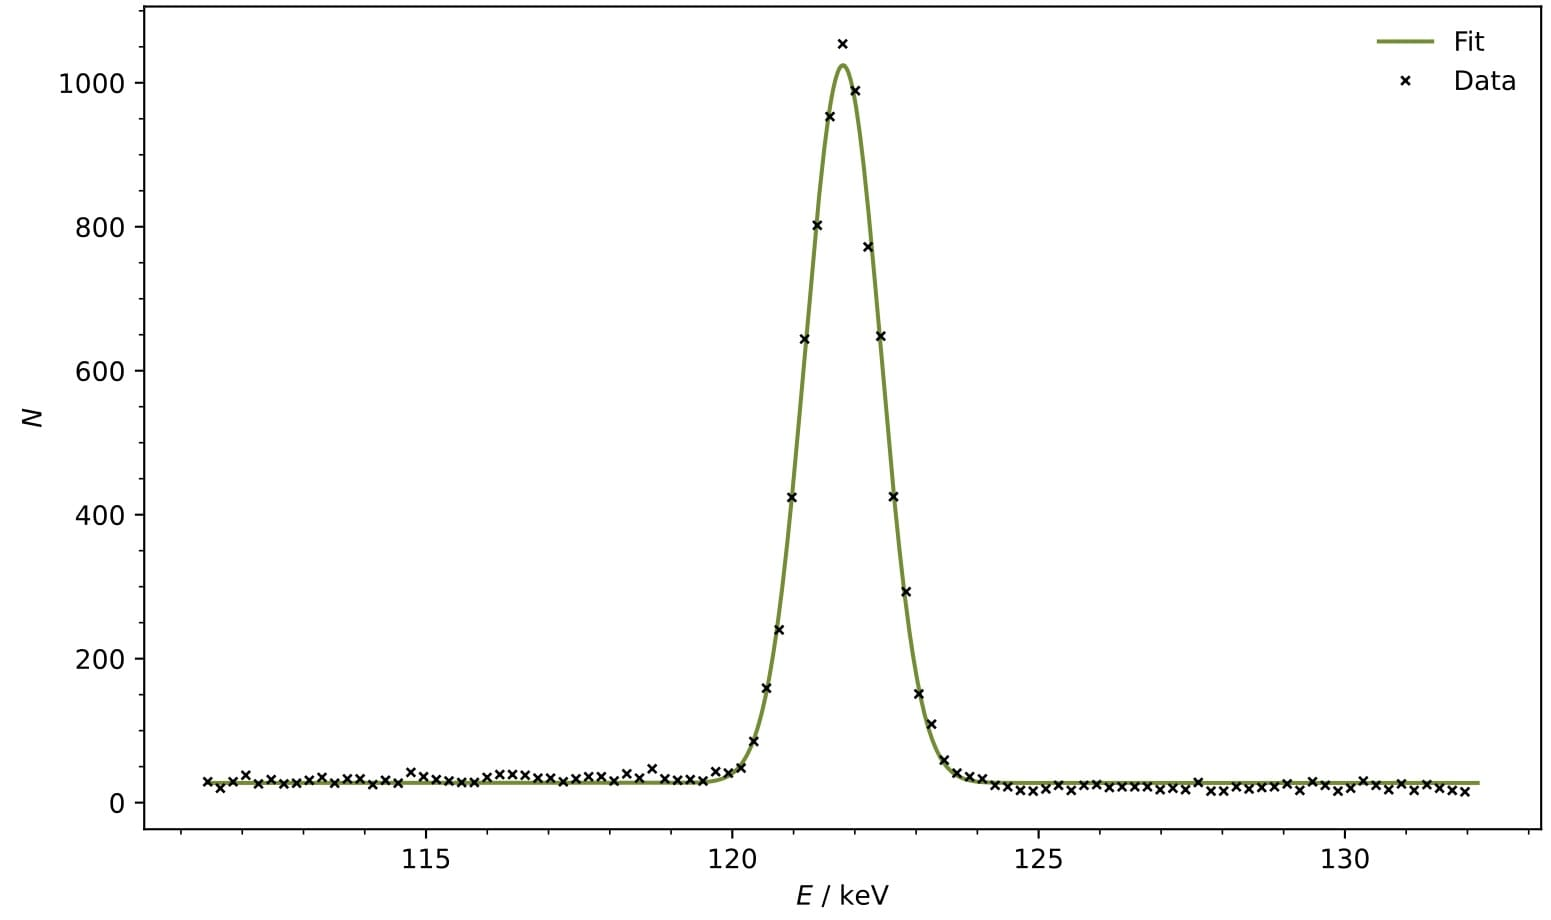
\includegraphics[width=0.8\textwidth]{content/plots/plot4.jpg}
   \caption{Fit einer Gaußkurve an einem Full Energy Peak für $E$ = \qty{122}{\kilo\eV} des Eu-152 Spektrums.}
   \label{fig:plot4}
\end{figure}

Es ist so möglich die Gesamtanzahl der Impulse pro Peak zu bestimmen zur weiteren Berechnung der Vollenergienachweiswahrscheinlichkeit.
Anhand des Fits kann auch der Hintergrund als konstant modelliert und durch subtraktion kompensiert werden.

Die Vollenergienachweiswahrscheinlichkeit wird mit der Gleichung 
\begin{equation*}
    Q = \frac{N}{AWt} \cdot \frac{4\pi}{\Omega}
\end{equation*}
bestimmt. $W$ Gibt die Emissionswahrscheinlichkeit an, A enspricht der Aktivität der Probe am Messtag (22.04.2024) und t
ist die Zeitspanne, über die gemessen wird.
Zur Bestimmung der Aktivität der Probe wird das Zerfallsgesetzt gemäß
\begin{equation*}
    N(t) = N_0 \exp(-\lambda t)
\end{equation*}
nach $t$ abgeleitet. Daraus folgt der Zusammenhang
\begin{equation*}
    A(t) = A_0 \exp(-\lambda t).
\end{equation*}

Die Aktivität am 01.10.2000 und die Halbwertszeit von Eu-152 sind geben durch
\begin{align*}
    A_0     &= \qty{4130+-60}{\becquerel} \\
    T_{\frac{1}{2}} &= \qty{4934}{\day}.
\end{align*}

Für den Tag der Messung (22.04.2024) ergibt sich eine Aktivität von
\begin{equation*}
    A = \qty{1233+-18}{\becquerel}.
\end{equation*}

Abschließen muss $\Omega$ berechnet werden und zwar anhand der Gleichung
\begin{equation*}
    \Omega = \frac{1}{2} \left(1- \frac{a}{\sqrt{a^2+r^2}}\right).
\end{equation*}

Dabei bezeichnet $a$ den Abstand der Probe zum Detektor, dieser beträgt in Summe \qty{85}{\milli\meter}.
Der Radius $r$ des Zylinders entspricht \qty{22.5}{\milli\meter}.